\documentclass[border=5pt]{standalone}
\usepackage{tikz}
\usetikzlibrary{arrows.meta,calc,decorations.pathreplacing}

\begin{document}
% Template: AD-AS multiplier effect
% Use for staged aggregate-demand shifts and final-output comparison.
% Math-logic gate: this template is schematic. For exact claims, generate
% AD/SRAS intersections from declared functions or data and attach guide lines,
% labels, and the output-change bracket to those computed coordinates.
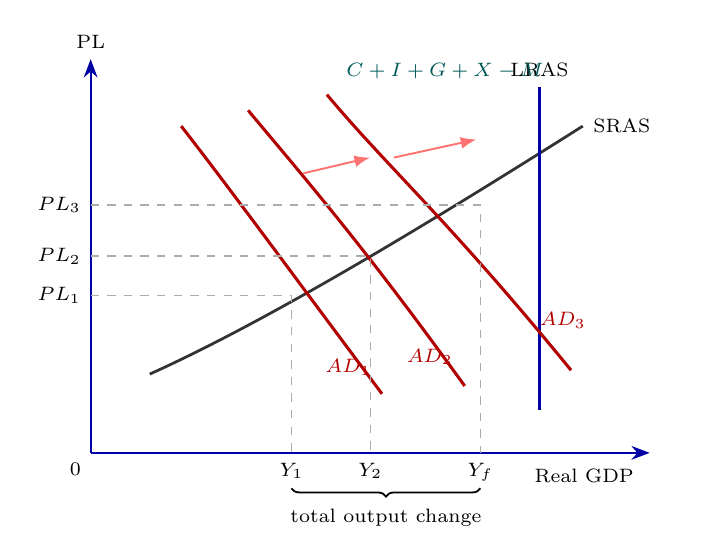
\begin{tikzpicture}[
  font=\sffamily,
  >=Stealth,
  axis/.style={->, draw=blue!65!black, line width=0.8pt},
  supply/.style={draw=black!80, line width=1pt},
  lras/.style={draw=blue!65!black, line width=1pt},
  ad/.style={draw=red!70!black, line width=1.1pt},
  guide/.style={draw=gray!65, dashed, line width=0.5pt},
  lab/.style={font=\scriptsize, align=center}
]
\path[use as bounding box] (-0.8,-1.0) rectangle (7.7,5.4);
\draw[axis] (0,0) -- (7.1,0) node[below left=2pt, lab, text=black] {Real GDP};
\draw[axis] (0,0) -- (0,5.0) node[above, lab, text=black] {PL};
\node[lab, anchor=north east] at (0,0) {0};

\draw[supply] (0.75,1.0) .. controls (2.3,1.7) and (4.35,2.95) .. (6.25,4.15)
  node[right, lab] {SRAS};
\draw[lras] (5.7,0.55) -- (5.7,4.65) node[above, lab, text=black] {LRAS};

\draw[ad] (1.15,4.15) .. controls (1.85,3.25) and (2.65,2.15) .. (3.7,0.75)
  node[pos=0.86, below, lab, text=red!70!black] {$AD_1$};
\draw[ad] (2.0,4.35) .. controls (2.75,3.45) and (3.45,2.65) .. (4.75,0.85)
  node[pos=0.88, below, lab, text=red!70!black] {$AD_2$};
\draw[ad] (3.0,4.55) .. controls (3.75,3.65) and (4.55,2.95) .. (6.1,1.05)
  node[pos=0.88, right, lab, text=red!70!black] {$AD_3$};

\draw[guide] (0,2.0) node[left, lab] {$PL_1$} -- (2.55,2.0) -- (2.55,0)
  node[below, lab] {$Y_1$};
\draw[guide] (0,2.5) node[left, lab] {$PL_2$} -- (3.55,2.5) -- (3.55,0)
  node[below, lab] {$Y_2$};
\draw[guide] (0,3.15) node[left, lab] {$PL_3$} -- (4.95,3.15) -- (4.95,0)
  node[below, lab] {$Y_f$};

\draw[-{Latex[length=2mm]}, red!55, line width=0.7pt] (2.7,3.55) -- (3.55,3.75);
\draw[-{Latex[length=2mm]}, red!55, line width=0.7pt] (3.85,3.75) -- (4.9,3.98);
\node[lab, text=teal!70!black] at (4.5,4.85) {$C+I+G+X-M$};

\draw[decorate, decoration={brace, amplitude=3pt, mirror}, line width=0.65pt]
  (2.55,-0.45) -- (4.95,-0.45)
  node[midway, below=4pt, lab] {total output change};
\end{tikzpicture}
\end{document}
